\begin{document}
%intro

A recent article by SVT Nyheter showed the season on the $1^\text{st}$ of November for different areas in Sweden, as can be seen in Figure \ref{fig:SVT}. According to this article it was already winter in the north of Sweden while in the most south part, including Lund, it was still summer. This did not seem to correspond to what one might observe when looking out the window in Lund, the ground was already covered with red leaves even though it was still summer according to SVT Nyheter. So which definition of the season are there and when do the seasons start in Lund. 

\begin{figure}[h!]
\centering
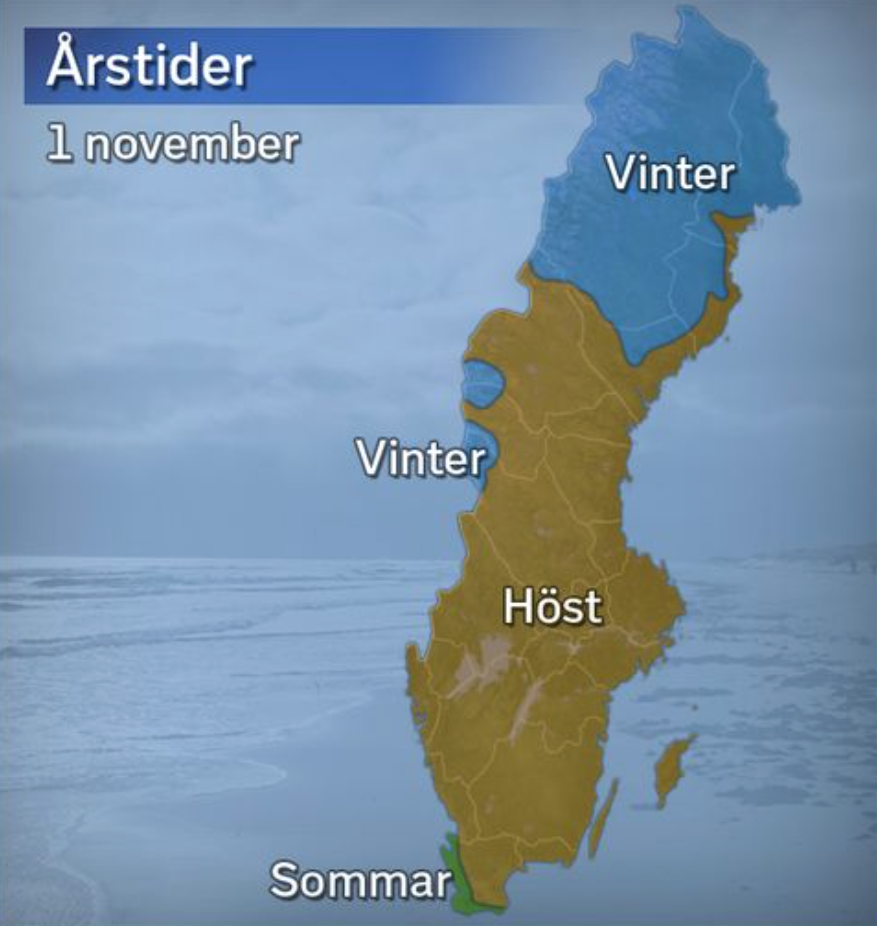
\includegraphics[width=0.4\textwidth]{SVT_seasons.png}
\caption{The season in different areas in Sweden on the $1^\text{st}$ of November. Image from \cite{SVT}.}
\label{fig:SVT}
\end{figure}

\subsection{Definition of the Seasons}
\cite{SMHI}


\subsection{Method}

\subsection{Results}
%The date is represented by the day of the year (i.e. from 1 to 365 or 366).

\begin{figure}[ht!]
\centering
\subfloat[Bar graph]{\label{fig:spring_bar}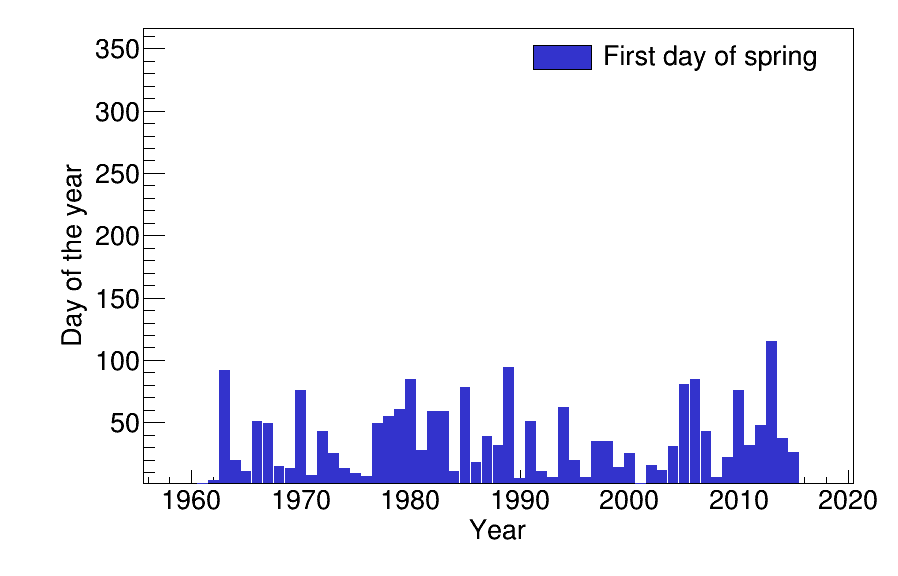
\includegraphics[width=0.5\textwidth]{springStart.png}} 
\subfloat[Histogram]{\label{fig:spring_hist}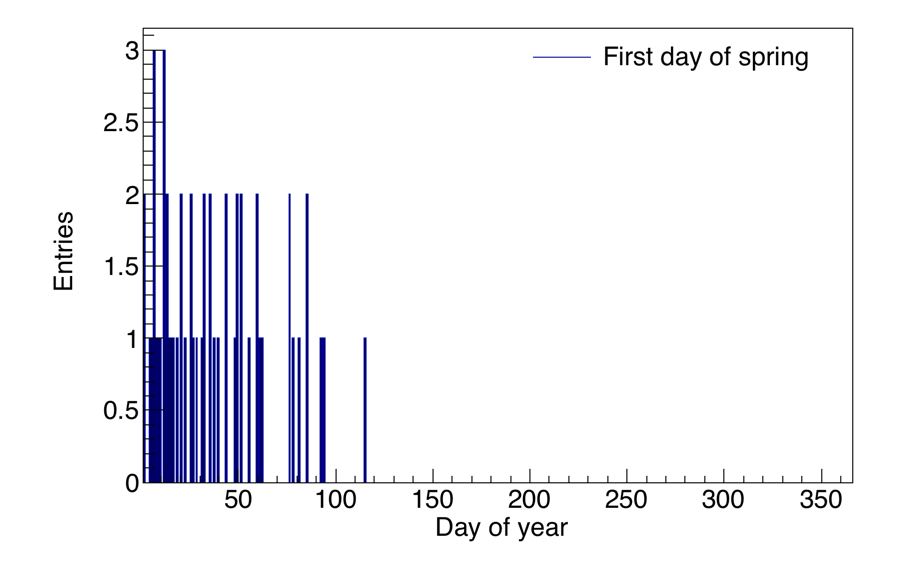
\includegraphics[width=0.5\textwidth]{springHistogram.png}}\\
\caption{The first day on which spring starts for each year in Lund is shown in (a).  While (b) shows the number of times spring starts on a certain day in the year.}
\label{fig:spring}
\end{figure}

\begin{figure}[ht!]
\centering
\subfloat[Bar graph]{\label{fig:summer_bar}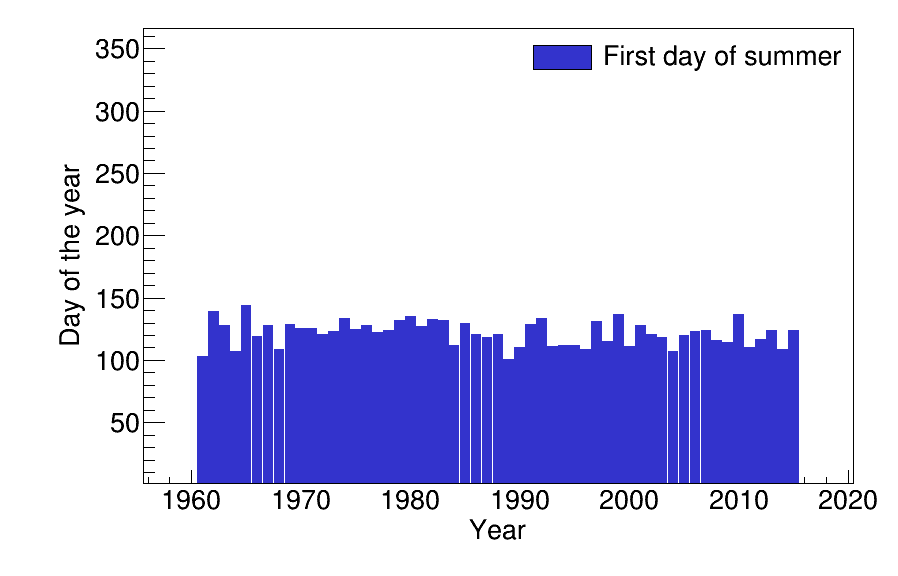
\includegraphics[width=0.5\textwidth]{summerStart.png}} 
\subfloat[Histogram]{\label{fig:summer_hist}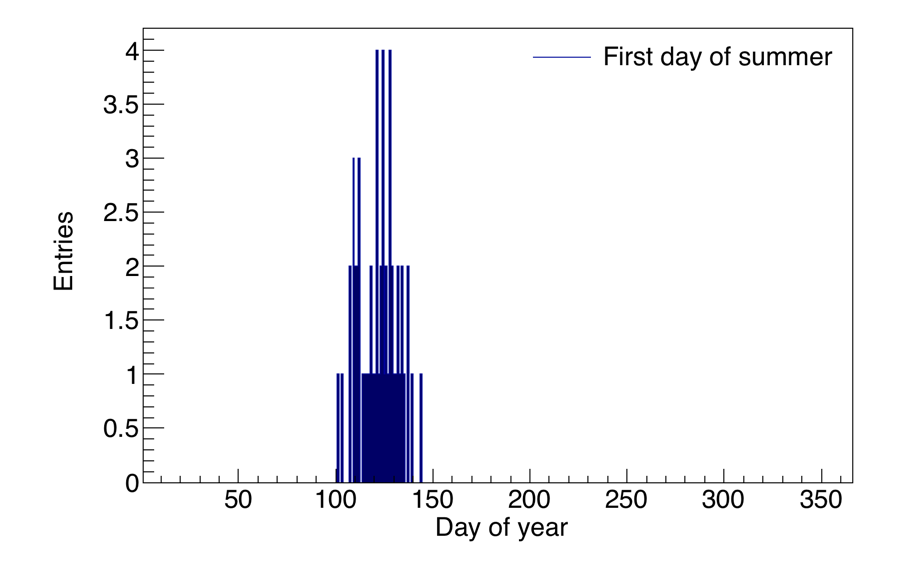
\includegraphics[width=0.5\textwidth]{summerHistogram.png}}\\
\caption{The first day on which summer starts for each year in Lund is shown in (a).  While (b) shows the number of times summer starts on a certain day in the year.}
\label{fig:summer}
\end{figure}

\begin{figure}[ht!]
\centering
\subfloat[Bar graph]{\label{fig:fall_bar}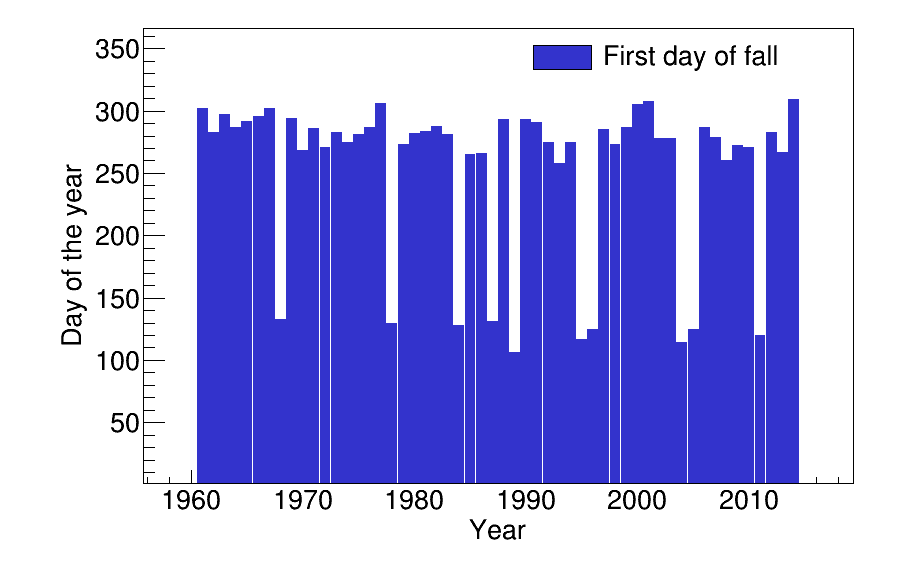
\includegraphics[width=0.5\textwidth]{fallStart.png}} 
\subfloat[Histogram]{\label{fig:fall_hist}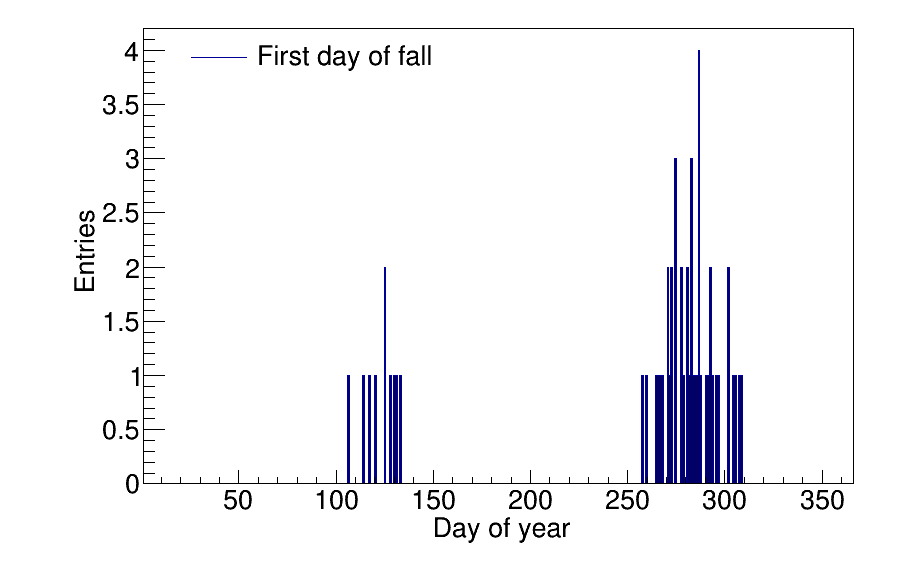
\includegraphics[width=0.5\textwidth]{fallHistogram.png}}\\
\caption{The first day on which fall starts for each year in Lund is shown in (a).  While (b) shows the number of times summer starts on a certain day in the year.}
\label{fig:fall}
\end{figure}

\begin{figure}[ht!]
\centering
\subfloat[Bar graph]{\label{fig:winter_bar}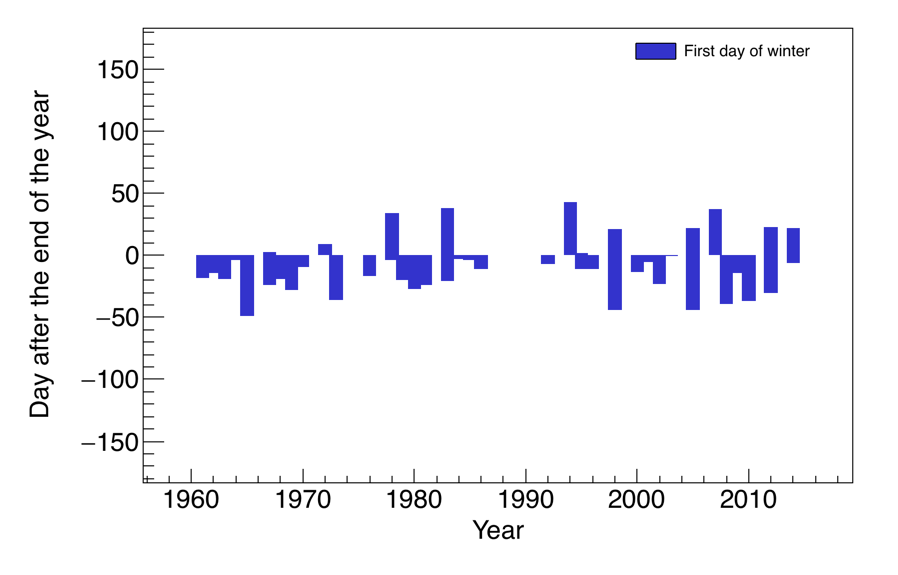
\includegraphics[width=0.5\textwidth]{winterStart.png}} 
\subfloat[Histogram]{\label{fig:winter_hist}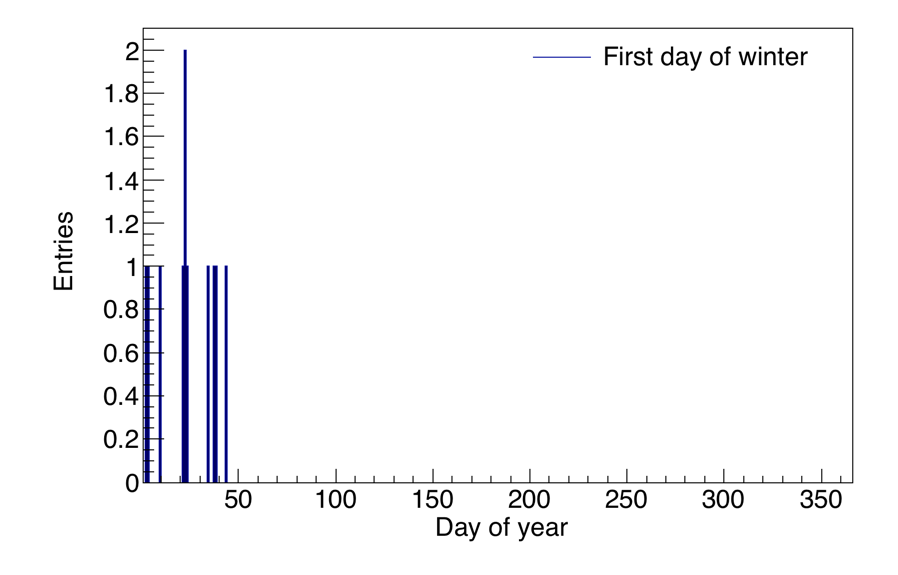
\includegraphics[width=0.5\textwidth]{winterHistogram.png}}\\
\caption{The first day on which winter starts for each year in Lund is shown in (a). The day is given relative to the start of a new year, all negative numbers are before the $1^{\text{st}}$ of January and all the positive numbers are on or after the $1^\text{st}$ of January.  The number of times spring starts on a certain day in the year in given in (b).}
\label{fig:winter}
\end{figure}

\end{document}















